\chapter{Prior and related work}\label{chapter_background_work}
Software Trajectory Analysis (STA) consists of two components: 
the \textit{software artifacts retrieval and measurement machinery} (i.e. a data assimilation layer), 
and the \textit{software trajectory characteristic patterns discovery module} (i.e. a data analysis layer). 
A high-level overview of the information flow through these components is show at the 
Figure \ref{fig:sta-full-overview}.

The artifacts retrieval and measurement machinery refers to a way that software artifacts are collected, 
measured, and enriched with metadata. 
Currently, STA is capable of retrieving and processing the data from OSS Software 
Configuration Management system (SCM) components such as version control, 
defect management, and communications management systems. 
In addition, STA is able to assimilate data from other data sources among which are community-driven 
Q\&A websites and the Hackystat system \cite{csdl2-10-09}.

STA is not limited only to these data sources.
As public repositories are highly heterogeneous and continuously evolving, STA adopts the 
Software Repository Mining (MSR) strategy for data assimilation, unification, and off-line enrichment,
where public artifacts are retrieved and stored ``\textit{as is}'' (i.e. mirrored) first, 
measured second, and enriched with metadata as the final step 
\cite{citeulike:12550438} \cite{german04_softchange} \cite{cvsanaly}.
Similarly to other systems for mining software repositories, STA relies on a relational database engine 
for data storage and indexing -- this solution not only enables an interactive workflow and a federated 
access to the data, but allows for effective measurements partitioning and aggregation, which is 
an \textit{essential capability} for efficient software trajectories construction.
Overall, the STA data assimilation layer is designed in a way that conforms to the field's best practices
allowing its extension for any data source that is capable of providing data for STA analysis.

The software trajectory characteristic patterns discovery module is an analytical machinery that 
is responsible for discovery of characteristic recurrent patterns in a set of software trajectories provided as 
the input. Conceptually, this module can embed \textit{any data mining algorithm} which is capable of 
discovering recurrent patterns from sequential data, such as one of the numerous algorithms for time series 
motif discovery \cite{citeulike:13197378}.

However, the specificity of software trajectories and the pattern of interest, i.e. recurrent behavior, 
places a number of constraints that limit the applicability of known algorithms.
First of all, the algorithm must be able \textit{to discover recurrent patterns without any prior knowledge 
about their length, shape, amplitude, and occurrence frequency}, as these are expected to naturally differ 
between projects, problems, or even subsets of trajectories from the same project.
Secondly, it must be capable to \textit{learn from a very small training data set} --
the property that has been shown crucial in predictive modeling and knowledge mining from software 
repositories where data is sparse \cite{citeulike:6055293}.
And finally, the algorithm must provide an automated mechanism for 
\textit{patterns ranking according to their relevance} in order to allow their efficient 
review by human experts since it is impossible to define a pattern ``interestingness'' or 
``importance'' a priori.

The STA characteristic patterns discovery module implementation relies on SAX-VSM,
a novel algorithm for characteristic patterns discovery from time series that I shall propose, describe, and evaluate 
in the Chapter \ref{chapter_sax_vsm}. 
This algorithm has been designed to address all of the aforementioned requirements.

\begin{figure}[t]
   \centering
   \includegraphics[width=150mm]{figures/Flow-analysis.eps}
   \caption{The high-level STA overview. Software artifacts are retrieved, enhanced, and measured within the
   data assimilation layer. Next, based on the user input, classes of software trajectories are constructed.   
   In turn, the data analysis layer performs comparative analyses of software trajectories that yield sets
   of ranked class-characteristic behaviors.
   Note, that for the clarity only two classes of trajectories shown whereas STA is capable of discovering
   class-characteristic patterns from many classes at once.}
   \label{fig:sta-full-overview}
\end{figure}

Later in this chapter, in order to relate Software Trajectory Analysis to other research and to position 
it among other work, I shall discuss previous work from several research areas.
To start, since STA is designed for software measurements analyses, I provide a background on software 
measurements and the evidence of their correlation with software processes. 
Next, I briefly discuss my earlier exploratory studies conducted with previous STA implementations. 
Finally, I review relevant to STA research from the Mining Software Repositories (MSR) research field 
focusing on recurrent behaviors discovery.
The work relevant to time series characteristic patterns discovery and SAX-VSM will be discussed 
in the next Chapter.

\section{Software measurements}
As in all other Engineering fields, measurements are used in Software Engineering in order to establish a 
systematic approach to software development which provides control over software processes, facilitates
their improvement, and, most importantly, makes their result predictable. 
In addition, software measurements enable the scientific research.

\subsection{Software measurement history}
According to Fenton \cite{citeulike:1525462}, the history of measurements in Software Engineering dates 
back to mid-1960's  ``\textit{...when the Lines of Code metric was used as the basis for measuring the 
productivity and effort...}'', which in fact, predates the establishment of Software Engineering as an 
independent discipline \cite{naur_crisis_68}. 
Much of early research concerned with software measurements has been driven by the need for the resource model 
prediction and forecasting \cite{citeulike:1525462}, whereas later research has extended towards the problem 
of software process management \cite{citeulike:13158802}.

Probably the earliest published work outlining close relations of software measurements and software 
processes is ``Software project forecasting'' by DeMillo and Lipton \cite{demillo1980software} where they 
point out that software measurements create a basis which allows practitioners and researchers to be 
``\textit{rational and objective}'' about software processes. 
Remarkably, the authors refer to even earlier notes by Perils, Sayward, and Shaw, who emphasized the role of software 
measurements in software process management, saying that ``\textit{the purpose of software metrics is 
to provide aids for making optimal choice at several points in the life cycle}''.

With time, the increasing understanding of software measurements objectiveness and their ability to reflect 
the state of software processes led to the development of measurement-based strategies for software 
process management and improvement. 
For example, one of the pioneering strategies for global software process improvement, 
Total Software Quality Management (TSQM), relies on a set of ten explicitly defined software 
process and product metrics ranging from the low level product metrics of Lines of Code and Design Complexity to 
the high-level project management metrics of Schedule and System Testing Progress \cite{citeulike:13071448}.
Similarly, a local strategy for the software process improvement, Personal Software Process (PSP), relies on 
the broad range of software metrics \cite{citeulike:13072239}.

In addition to playing an important role in software process management and forecasting, software 
measurements have become ubiquitous in scientific research. 
For example in the research field of Empirical (or as it also called Experimental) Software Engineering (ESE), 
researchers use measurements and experimentation as the basis for research hypotheses 
generation and their investigation \cite{citeulike:766768}. 

Recently, due to the proliferation of open source software development and advancements in public software
project hosting solutions, a new research area called Mining Software Repositories (MSR) has been established 
within ESE field. MSR is specifically concerned with application of analytical techniques to public software 
repositories \cite{citeulike:12550438} \cite{citeulike:4534888} \cite{citeulike:2710928}, thus, 
the research work from this field is one of the most relevant to my research.

\subsection{Software measurement theory}
In science and in engineering, measurements allow us to formally characterize attributes of an entity by assigning 
them a numerical, boolean, or symbolic value. 
The choice of the value type depends on the measurement criteria, such as a dimension, a level, 
or a degree. Ultimately, the chosen criteria and the scale of used values shall enable an intuitive 
and precise quantitative comparison between attributes regardless of their qualitative similarity or 
difference, as it was pointed out by Chapin \cite{citeulike:13158806}. 
In addition, measurement units and scales are usually standardized in order to enable a global comparability.

An entity in Software Engineering can be a physical object, such as a program or a use case diagram, 
an event, such as a software release, or a software artifact, such as a bug report.
A measurable entity's attribute can be its property or a feature, such as the program's size, the 
amount of defects discovered during testing, or the usability of a software system.

Further, attributes are usually divided into two categories: internal and external. 
While measures for internal attributes are computed based on the entity itself, external attribute 
measures depend on both the entity and the environment in which it resides -- for example a 
software system testing time varies depending on the performance of a test server.

Finally, as pointed out by Fenton \cite{citeulike:1803429}, there are two broad types of measurements: direct
and indirect. While direct measurements of an attribute do not depend on any other attributes, 
indirect measurements involve measurements of one or more other attributes. 
As an example of a direct measurement, consider the size of a system source code or the time developers spent 
on project. In contrast, the module defect density (ratio of defects number and the module size), 
or the requirement stability (ratio of initial requirements and total requirements) are indirect measurements.

\subsection{Software measurements in STA}
Software Trajectory Analysis is designed for analyses of software measurements in order to enable 
recurrent behaviors discovery. In particular, STA exploits the sequential dependency of consecutive 
measurements for discovering recurrent characteristic patterns in their dynamics (i.e. structural patterns), 
which, as I hypothesize, reflect recurrent behaviors.

\begin{figure}[t]
   \centering
   \includegraphics[width=115mm]{figures/SEI-measurements.eps}
   \caption{The illustration of relations between software measurements and key responsibilities 
   in project management from SEI Guidebook \cite{citeulike:10567306}. Note, that product and process 
   measurements are the only input into the analyses and the process control blocks.}
   \label{fig:sei-measures}
\end{figure}

This approach builds upon previous work that confirmed the feasibility of software processes inference through 
observations (i.e. measurements) of their effect on software product evolution and indicated the possibility of 
recurrent behaviors discovery. 

As an specific example, confirming the observability of software processes through software product measurements, 
consider the de-facto industrial standard for software measurements application provided by 
Software Engineering Institute (SEI) in their guidebook \cite{citeulike:10567306}. 
In particular, the authors focus on the software process execution variability issue that significantly 
affects the software project's schedule and the resulting software system quality. 
To address the issue, they propose a methodology based on implementation of a continuous software product 
and process measurement program, that allows for continuous assessment of the software processes 
variability enabling a ``real-time'' software process control. 
Figure \ref{fig:sei-measures} illustrates their approach.

Hackystat, the ``parent'' system of STA, is another relevant study that extends the applicability of continuous 
measurements and confirms the possibility of software process understanding through the analysis of recurrent 
behaviors \cite{citeulike:557296}. 
As pointed out by the authors, the visual comprehension of measurements variability and pattern collocations enables 
``\textit{emergent knowledge that one state variable appears to co-vary with another in the current project context}'',
allowing for process improvement activities \cite{citeulike:557296}. 

As an example indicating the possibility of recurrent behaviors discovery through measurements, consider the 
study by Hindle et al. \cite{citeulike:10377345} discussed in the Section \ref{chapter2_section-tsanalysis} of 
this chapter that proposes a methodology for recurrent behaviors detection based on Fourier Transform analysis.

STA extends previous approaches built for software measurements analysis by providing an automation for 
characteristic patterns discovery from software process and product measurements, which, as I expect, shall 
aid in understanding of recurrent behaviors and their role and effect in software processes.

\section{Mining Software Repositories}
As mentioned before, mining software repositories is a well established research direction since 
mid-1970's, when Meir Lehman pioneered the software evolution theory by studying historical records from 
software repositories \cite{citeulike:2739216}. 
For the last decade, researchers working in the field discuss their approaches and findings in a number of venues. 
Among these are the Predictive Model in Software Engineering (PROMISE) workshop and the Working Conference on Mining 
Software Repositories (MSR) which are held within the annual International Conference on Software Engineering (ICSE)
and specifically focus on the analysis of software repository artifacts.
In order to enable the comparison of proposed techniques performance, both venues encourage researchers to 
apply them to reference datasets. 
While PROMISE maintains the same reference dataset over years \cite{promise12}, 
MSR offers a so-called MSR challenge dataset annually \cite{MSRChallenge2012} \cite{MSRChallenge2013}.
Note however, that the {PROMISE} research is mainly concerned with the development of predictive models for 
Software Engineering \cite{Menzies13}, whereas MSR traditionally uses data from public software repositories stimulating 
the diversification of research directions \cite{citeulike:12550438} \cite{citeulike:2710928} \cite{citeulike:7853299}.

\section{Understanding Public Software Repositories}\label{section_understanding}
Traditionally, software repositories contain a variety of artifacts produced during the software life-cycle
and can be categorized by their purpose.
Previous research assigns software repositories into three main categories: source code control, 
defect tracking, and archived communications systems \cite{citeulike:4534888}, but other types of repositories exist. 
These may contain various information, such as software system runtime logs, system testing logs, 
historical measurements, documentation, tutorials, etc.
Recently, a novel type of repositories was proposed for MSR studies -- a historical information collected within the 
community-based question answering service Stack Overflow \cite{MSRChallenge2013}.

As pointed out in previous review studies \cite{citeulike:12550438} \cite{citeulike:7853299} \cite{citeulike:7465518} there
are a number of issues associated with mining of \textit{public} repositories which not only create technical difficulties for 
scientific research, but also affect its validity. 
The chief problem is that public project repositories are highly heterogeneous - each is managed and operated 
mostly in isolation serving a particular project and community needs, therefore having no explicit interactions with 
other projects. 
Furthermore, within a project's repository, its SCM subsystems such as version control, defect-tracking, and mailing list, 
are rarely ``connected''  \cite{citeulike:13058334}. 
This issue of heterogeneity directly affects MSR studies generality since tools working for and results obtained from 
one repository, are rarely applicable to another.
Yet another issue is that while the public availability of software artifacts mitigates observability and privacy issues, 
the nature of these artifacts creates a number of other challenges which limit the possible scope of the scientific 
research and significantly elevate its complexity. Among others, four issues are usually cited as the most significant:
\begin{itemize}
 \item First of all, the artifacts are created by developers and users not in order to enable scientific research,
but rather to support software development activities. Therefore, the informational content of these artifacts is rather 
poor and additional evidence (i.e. metadata) is often needed \cite{citeulike:342840} \cite{citeulike:7954249} 
\cite{citeulike:7260421}.
 \item Second, the majority of these artifacts (change records, defect reports, assigned tasks, etc.) 
typically represent a snapshot of the software project state rather than reflect any of the performed actions.
Thus, it might be simply impossible to infer complete software development processes \cite{citeulike:1296888}.
Also, this fact effectively renders unusable (within public MSR domain) most if not all of previously developed 
event-based process and behavior discovery tools as their starting point is an event log \cite{citeulike:12944447}.
 \item Third, the project's contributors not only create and submit artifacts to repositories on their own volition,
but most of change management systems (such as Git, Subversion, and Gerrit) encourage the asynchronous workflow 
where the locally created artifacts may remain uncommitted and therefore unaccounted for as it has been shown previously
\cite{citeulike:2280690} \cite{citeulike:9037939}. 
For the same reason, it is often impossible to know \textit{exactly when} the artifact's content was created.
 \item Finally, the vast volume of produced artifacts, their high dimensionality, and significant noise demand 
 for automated, high throughput and robust analysis techniques 
 \cite{citeulike:12550438} \cite{citeulike:7853299} \cite{citeulike:4534888} \cite{citeulike:7549051}.
\end{itemize}

These issues not only create significant external threats to MSR research validity, but usually are \textit{impossible to resolve}
without altering the normal flow of OSS software process, for example by implementing a special measurement program, 
or by introducing instrumented source code editors and development tools (as in Hackystat). 
Typically, MSR researchers deal with them by seeking for additional evidence in order to support their conclusions 
\cite{citeulike:5043664} \cite{citeulike:5128808}.

\subsection{Public software artifacts}
Public software repositories offer a wide range of software process and product artifacts for analyses.
Among others, these include source code change records, defect reports, feature requests, accepted, 
rejected and assigned tasks, developer communications, documentation, tutorials, etc. 
All these allow developers and users to instantly obtain a ``snapshot'' of the project, i.e. to retrieve the 
latest (or any previous) source code revision and a complete overview of the software project state,
along with the lists of open and closed issues, past and future plans, and other information.

However, while being exceptionally convenient for the project participants, users, and management, this 
snapshot-oriented nature of public software artifacts creates numerous difficulties for software process research 
as a ``snapshot'' rarely reflects finished, ongoing, or planned processes -- the issue that limits the feasibility and 
compromises the validity of performed studies as I have mentioned above. 

I acknowledge this software process observability problem when working with public software process artifacts 
and intentionally avoid discussing and concluding on software processes. Instead, what I shall focus on in this dissertation, 
is the validation of the proposed technique's ability to capture process-characteristic recurrent behaviors when snapshots 
are viewed in their dynamics. 

Nevertheless, I hypothesize that in addition to the fact that the evolution of software measurements in time reflects 
recurrent development behaviors, some of these can be characteristic of certain aspects of software processes. 
Therefore, by discovering recurrent patterns in the evolution of software measurements it shall be possible to at least 
partially infer and evaluate performed software development actions or processes.

Further in this section I review a number of common public software repositories and their artifacts to whose measurements 
STA already has been or potentially can be applied. 

\subsubsection{Source code management system}
Source code management systems keep track of the main output of a software project -- its source code, which is also the 
main subject of scientific research. Metrics derived from the source code artifacts are predominant in studies concerned 
with software evolution, complexity, maintainability, and quality, as well as those that are concerned with productivity, 
project planning, and cost estimation (i.e. management) \cite{citeulike:4534888}. 

Typically, the evolution of source code is recorded as a sequence of consecutive change records, which are simple artifacts
tracking the change of each source code line. Despite the artifact's simplicity, tracing source code evolution through 
the analysis of change records can become increasingly difficult as developers branch the source code tree, merge it back, 
or abandon branches \cite{citeulike:13156191}.

While a large number of metrics can be derived through source code and change records analyses, it offers probably 
the most functional one -- the count of physical lines of code (LOC). Other source code metrics, such as the count of logical lines 
of code (LLOC), function points (FP), or software system complexity are much less used as they are language-dependent and their 
derivation involves significant data processing overhead.

\subsubsection{Defect tracking system}
Normally, the software project defect repository serves as a centralized system for managing all of software project 
Quality Assurance (QA) activities providing users and developers with a means to report and to discuss improper system 
behavior.
In some projects, the defect repository is also used to keep a track of requests for future system features and related
discussions.

Artifacts from defect repositories are numerous and complex, as they may contain system logs, input and output files, 
screen-shots, etc. Their main purpose is to provide users with up to date information about system defects, their severity, 
and, if implemented in the system, with additional information about their technical nature and resolution plans.

By studying defect records, researchers can address many research questions which are concerned with software quality,
developer's expertise, and the project's technical debt \cite{citeulike:12550438}. 
In addition, defect records are traditionally used for predictive modeling.
For example, the ability to build predictive model for future bugs by their association with source code file change patterns 
(i.e. activity) has been shown by Zimmermann et al. in \cite{citeulike:6055293}, whether Livshits \& Zimmermann 
have shown a defect predictive model based on characteristic code fragments \cite{citeulike:393158}. 
An interesting approach for software testing processes optimization based on the identification of source code 
``hot spots'' through mining of the bug reports history has been shown by Ostrand \& Weyuker in \cite{ostrand2004tool}.

\subsubsection{Developer communications}
As OSS projects are usually developed by distributed teams that typically lack the ability for face-to-face meetings, 
emails, mailing lists, and newsgroups are used as primary communication channels between project participants. 

Developer communications artifacts, such as email messages, mailing list posts, and newsgroup messages include 
agent identification, timestamps, topics, and other data, that provide information allowing for not only process agents 
identification, but also understanding of their actions and process coordination activities (i.e. roles). 


For example Ying et al. in \cite{citeulike:1366052} proposed an interesting research direction of mining developer 
communications content for understanding of software quality, while Huang et al. in \cite{citeulike:9495129} used developer 
communications to build a developer interaction network and to partition developers by level of their involvement into the 
project or by technical expertise.

\subsubsection{Q\&A websites}
Frequently, professional software developers, amateur programmers, and computer hobbyists seek answers to various questions 
using the Internet. 
Among others resources, the Internet offers com\-munity-driven platforms, such as the Stack Overflow (SO) website that explicitly 
targets programmers and is dedicated to software-, hardware-, and computer system administration-related issues.

While other types of artifacts available, the ones distributed by SO team are probably the most used in the MSR research. 
These are distributed monthly and contain the historical information about questions and answers along with their change 
history including voting data. In addition, the SO team provides rich metadata about their service contributors. 
The public Stack Overflow dump was selected as the reference dataset in recent 2013 MSR Challenge \cite{MSRChallenge2013} 
which collected a number of submissions proposing interesting data analysis approaches.

While many of these are concerned with programming-related questions, such as identifying topics relevant to particular 
development communities \cite{kartik:msr14}, mining additional technical expertise \cite{VenkataramaniGAMB13} \cite{SaxeMG13}, 
or identifying problematic APIs \cite{KavalerPGCDF13} \cite{Linares2013Exploratory} and documentation \cite{Campbell2013Deficient},
some studies address broad phenomena such as collaborative problem solving \cite{Tausczik2014Collaborative},
knowledge sharing \cite{VasilescuCSCW14} \cite{Schenk2013Geo}, and contributor behaviors \cite{Bosu2013Building} \cite{GinscaP13}.

\subsubsection{Metadata}
Often, as reported by Begel et al. \cite{citeulike:7260421} who conducted a survey at Microsoft, in order to understand 
performed software processes, quantitative information about source code change is not sufficient. 
Through the survey, the authors accounted for 31 types of informational needs necessary for understanding and 
coordinating software processes, among which the need for the software change metadata was clearly articulated. 
Amid other reasons, it was found that metadata allows developers to learn the rationale behind software change,
find responsible people, discover and track dependencies, and to learn about the status of items in progress. 
The authors concluded that the majority of developer needs were concerned with people, not the code, and that 
metadata is essential in meeting these requests.

Similarly, Kim et al. \cite{citeulike:4000311} proposed a system for software repositories data collection, storage, 
and a universal data-exchange language and emphasized the importance of metadata for information management.
In addition, the authors showed that it is possible to create a public, metadata-centric system for interfacing 
closed-source software repositories to public open-source repositories.

Based on these and other results, I have designed the STA database storage in an extensible metadata-centric manner. 
New types of metadata can be defined by the user and associated with existing and newly collected artifact entities 
and measurements. In turn, within the process of software trajectories definitions, the metadata allows for efficient 
data partitioning and retrieval.

\section{Data assimilation}
Currently, there is a voluminous amount of research literature that deals with mining of public software repositories 
\cite{citeulike:2710928} which, in fact, extends an even larger body of research work that covers studies based on mining 
private software repositories and databases \cite{citeulike:393158} \cite{citeulike:13125375} \cite{citeulike:13125481}.

While the majority of published work is concerned with analyses of a repository information 
for better understanding of software systems evolution \cite{citeulike:277045} \cite{citeulike:4000311}, 
understanding and improving software processes \cite{citeulike:5803126}, 
and with studying the impact of software tools on the processes and products \cite{citeulike:13125389},
some effort has been made towards automation of the historical data retrieval, measurements, and its representation. 
A number of the proposed solutions allows for the real-time interactive repositories exploration implemented by extending 
repository management tools such as CVS, SVN, etc. with a front-end engine, such as Bonsai \cite{bonsai},
or JReflex \cite{citeulike:3017440}, while others, such as CVSAnalY \cite{citeulike:6544724}, 
softChange \cite{citeulike:13125395}, and {TA}-{RE} \cite{citeulike:4000311} propose an approach based on 
the off-line artifacts retrieval, pre-processing, and on-demand analysis.

\begin{figure}[t]
   \centering
   \includegraphics[width=115mm]{figures/Flow.eps}
   \caption{Detailed overview of the Software Trajectory Analysis data assimilation layer. 
    At first, software artifacts are mirrored from software repositories, measured, converted into 
    universal to STA format by repository-specific parsers, and stored in the dedicated relational database.
    In turn, stored in STA DB entities can be further enhanced with additional measurements and metadata.}
   \label{fig:sta-assimilation}
\end{figure}

Similarly to the latter, STA relies on the off-line retrieval, mirroring, and pre-processing of public software artifacts as
shown at the Figure \ref{fig:sta-assimilation}. Note, that since STA has been initially designed as a Hackystat extension 
\cite{csdl2-10-09}, it does not need any specific parser and is capable of real-time collection of Hackystat data.

\section{Relevant MSR research on recurrent behaviors discovery}
As I have shown above, MSR is a very diverse research field concerned with a variety of problems. 
%Among others, researchers use information extracted from repositories to address research questions related to software system growth, 
%its understanding, software quality prediction, refactoring and change patterns, measuring individuals expertize and contribution,
%understanding development teams social structure, and with software processes understanding.
But in this section I focus on previous MSR work that is specifically concerned with the application of analytical 
techniques to sequences of software artifact measurements -- the approach that STA builds upon.

\subsection{Itemset mining}
In data mining, frequently occurring items (actions, events) are often used in order to discover implicit knowledge from
large datasets. As I have mentioned earlier in Section \ref{section_software_process_design}, techniques based on frequent
items mining were previously applied for software process discovery from development event logs 
by Cook and Wolf \cite{citeulike:328044} \cite{citeulike:5120757} \cite{citeulike:5128143} 
and by Rubin et al. \cite{citeulike:1885717}. Unfortunately, since public software repositories do not offer 
development event logs \cite{citeulike:1296888}, these techniques can not be adopted for mining software 
repositories in their proposed form.

Nevertheless, sequential item mining has found a number of applications in MSR.
For example Zimmermann et al. in \cite{citeulike:277045} developed a system called ROSE for the identification of 
co-occurring changes in a software system that aids in future change prediction. 
For the same purpose, Kagdi et al. \cite{citeulike:3929070} developed a sequential pattern mining technique capable of 
discovery of ordered sequences of frequently changed files. 
Livshits \& Zimmermann \cite{citeulike:393158} developed DynaMine -- the system for bug prediction based on mining 
of frequent function call patterns.

Potentially, itemset mining  techniques can be applied to STA results. For example it may be possible to discover ordered, or
unordered sequences of recurrent behaviors which can be further associated with particular development actions.

\subsection{Time series analysis}\label{chapter2_section-tsanalysis}
Because the majority of software artifacts are time stamped, some MSR research seeks to quantitatively analyze ordered 
in time sequences of software artifacts or their measurements as these may carry useful information about software 
processes and recurrent behaviors. 

\begin{figure}[t!]
   \centering
   \includegraphics[width=145mm]{figures/FourrierMySQL.eps}
   \caption{Figures from the study by Hindle et al. \cite{citeulike:10377345} confirming the existence of periodicity
   in daily changes (left panel) and the possibility of their frequency discovery using Fourrier transform (right panel).   
   }
   \label{fig:mysql-fourrier}
\end{figure}

For example Herraiz et al. \cite{citeulike:6544685} applied Autoregressive Integrated Moving Average (ARIMA) model 
to software evolution measurements for prediction of future changes. The authors has shown that it is possible to 
predict a number of future changes in Eclipse by the means of resulting non-explanatory statistical model. 

Similarly, Antoniol et al. \cite{citeulike:3378725} have explored the application of a common signal processing toolkit 
built upon Linear Predictive Coding (LPC) and Cepstrum coefficients to modeling of software artifact histories. 
In particular, the authors have shown that it is possible to identify files with very similar size change histories 
by using the proposed approach.

The temporal segmentation of time series has been applied to mining of Eclipse change log by Siy et al. \cite{citeulike:10896305}.
The authors have demonstrated that by partitioning of continuous development activities into the smaller segments whose duration 
is close to the software release cycle, it is possible to discover ``stronger trends'' (i.e. characteristic behaviors). 
For example they have found that developers tend to focus on a particular file subset within a release cycle duration. 
In addition, they were able to detect similar change activity patterns among developers.

Finally, Hindle et al. in \cite{citeulike:10377345} outlined an approach for discovery of recurrent behaviors from software 
measurements by Fourier analysis. 
The left panel of the Figure \ref{fig:mysql-fourrier} from their work indicates that the studied signal carries potentially 
distinguishable periodic behaviors, moreover, they were able to detect a promising smear of frequencies between 18 and 19 
[days] as it is shown at the right panel. Unfortunately this direction was not further investigated.

\section{Summary}
In this chapter I have reviewed the most relevant to my work previous contributions to the fields of Software Project Management 
and Mining Software Repositories. Specifically, I have provided the evidence for a tight correlation between product and process evolution 
and their measurements that enables my research, showed relevant previous work which indicate its feasibility,
and enumerated challenges associated with mining of software repositories that shape STA design. 

In addition, I have discussed my experiences with earlier STA implementations which confirmed a satisfactory performance of 
the proposed approach based on measurements partitioning and their symbolic discretization that mitigate for the lack of baselines 
and noise respectively. Note that at the same time, previous STA experimentation revealed the demand for a new analytical technique 
that is capable of unsupervised characteristic patterns discovery and ranking. In the next chapter I show a technique called SAX-VSM 
that addresses the demand and enables unsupervised characteristic patterns discovery from time series.

\epigraph{Without the right information, you're just another person with an opinion.}{Tracy O'Rourke, CEO of Allen-Bradley}